\begin{figure}[h]
    \centering
    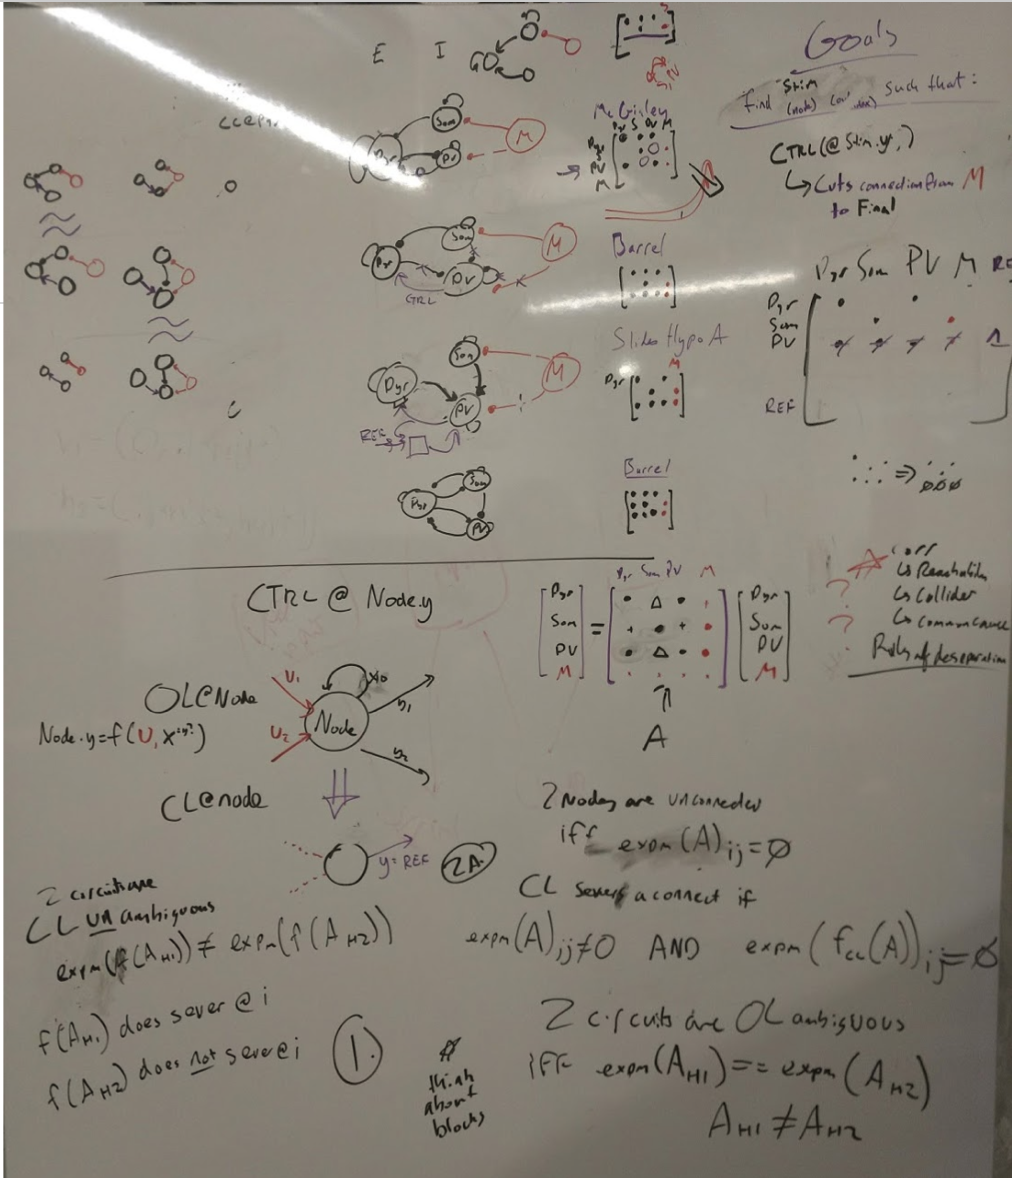
\includegraphics[width=\textwidth]{big_circuit_wb.png}
    \caption{Circuit diagrams}
\end{figure}

\begin{figure}[h]
    \centering
    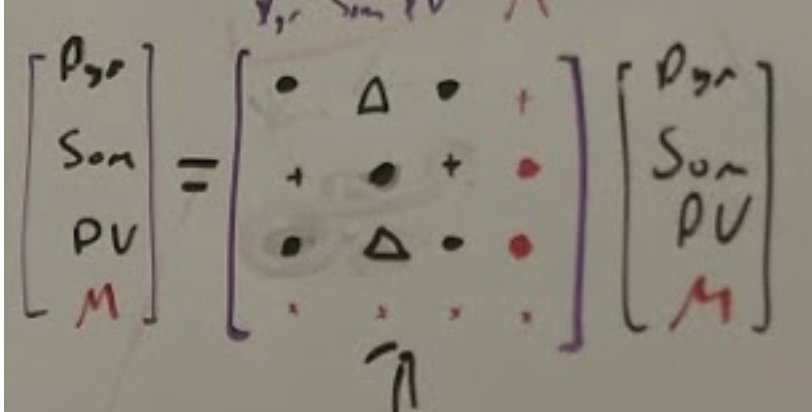
\includegraphics[width=\textwidth]{just_adj_mat.png}
    \caption{Linear representation of functional model}
\end{figure}

\begin{figure}[h]
    \centering
    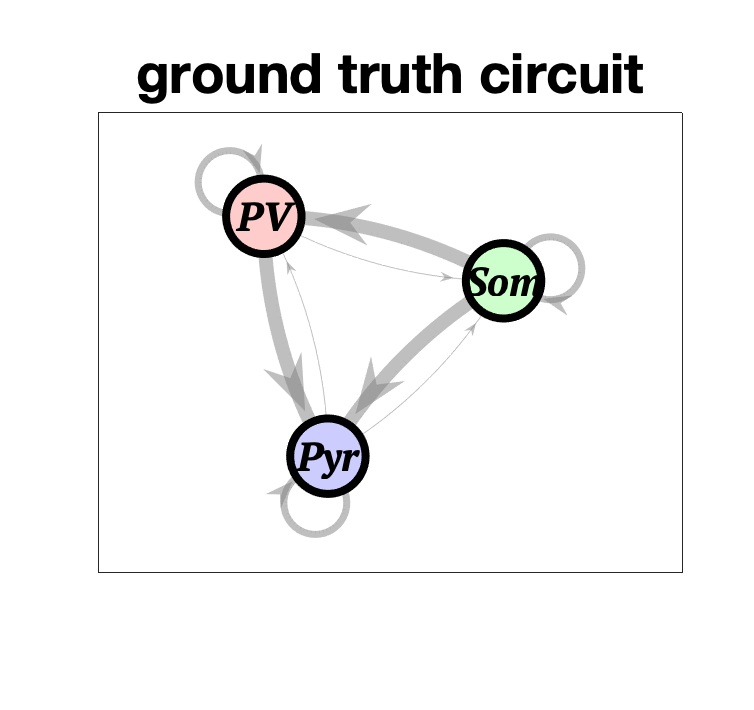
\includegraphics[width=\textwidth/2]{obsv_graph.png}
    \caption{graph representation of cortical circuit}
\end{figure}

\begin{figure}[h]
    \centering
    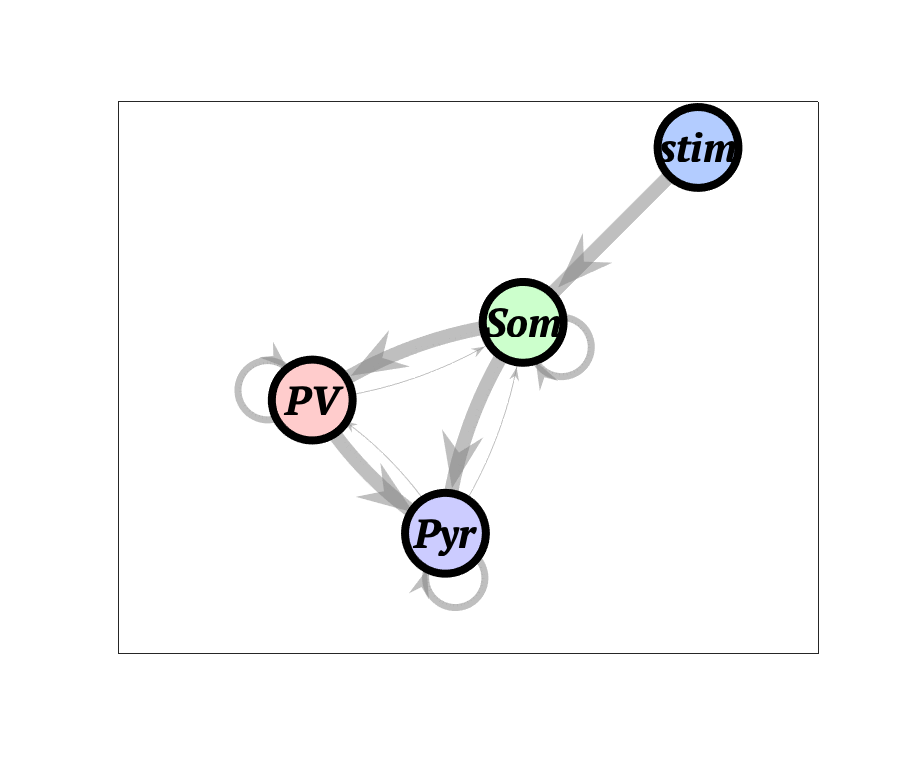
\includegraphics[width=\textwidth/2]{ol_graph.png}
    \caption{graph representation of open-loop control applied to cortical circuit}
\end{figure}

\begin{figure}[h]
    \centering
    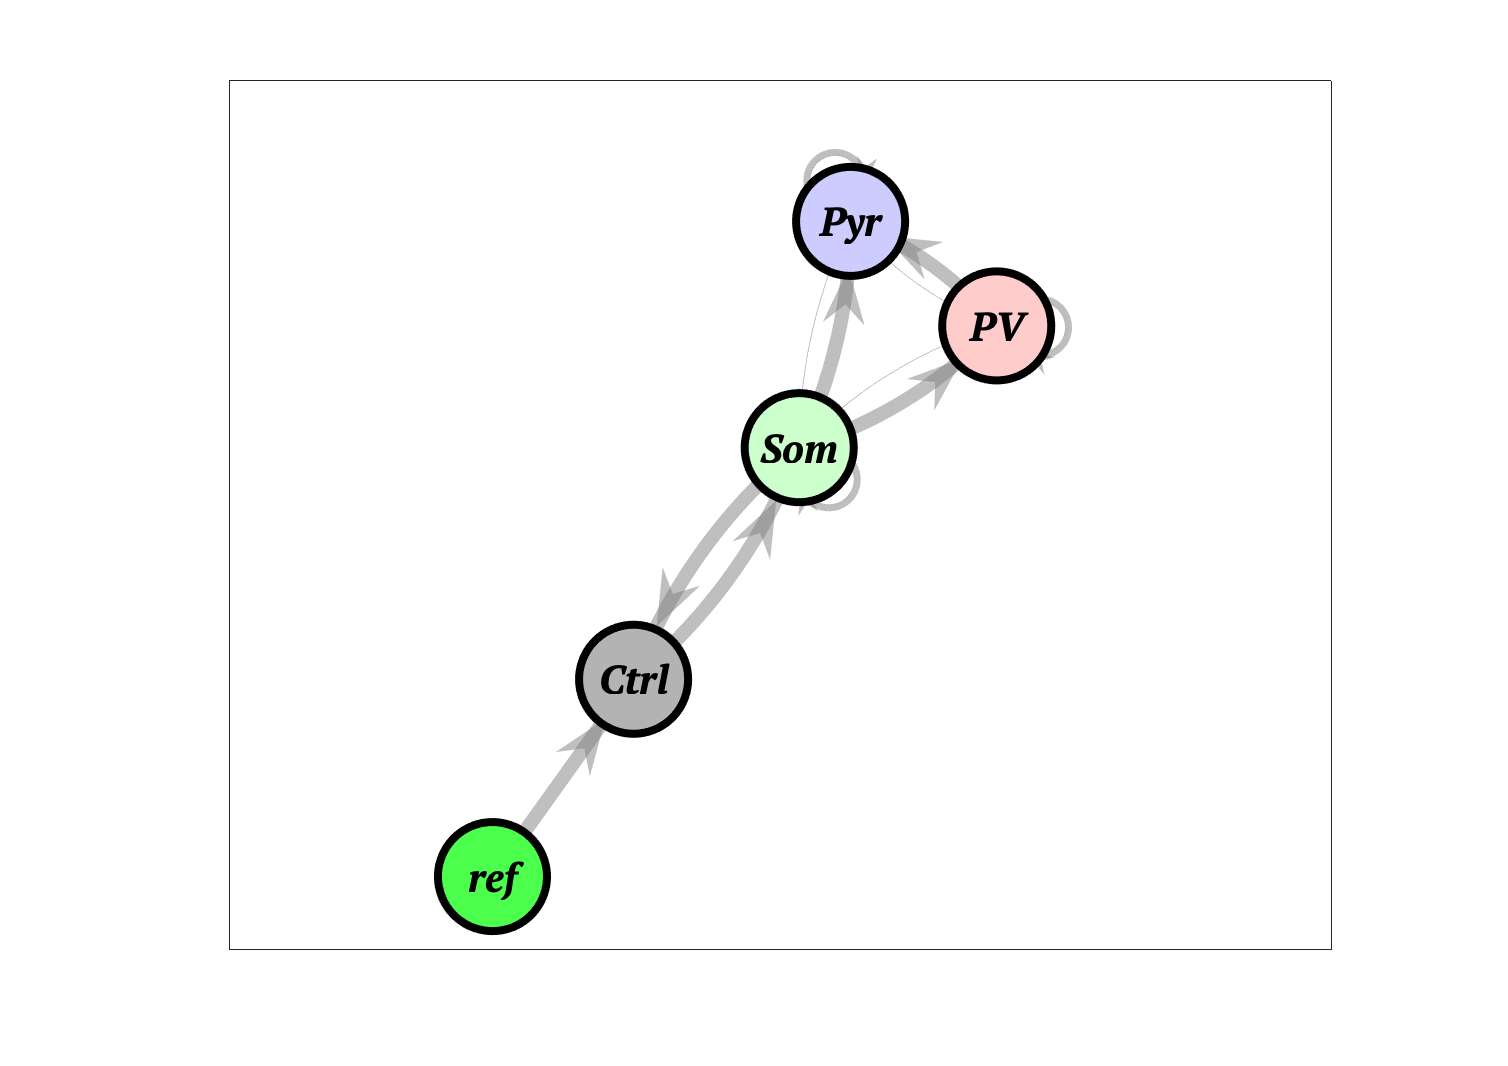
\includegraphics[width=\textwidth/2]{cl_graph.png}
    \caption{graph representation of closed-loop control applied to cortical circuit}
\end{figure}

\begin{table}[h!]
    \centering
    \begin{tabular}{|c|c|c|c|c|c|}
     \hline
     \begin{bmatrix}
     1 & 1 & 1\\
     0 & 1 & 0\\
     1 & 0 & 1
     \end{bmatrix}
      & 
     \begin{bmatrix}
     1 & 1 & 1\\
     1 & 1 & 0\\
     1 & 0 & 1
     \end{bmatrix}
      & 
     \begin{bmatrix}
     1 & 1 & 1\\
     0 & 1 & 0\\
     0 & 0 & 0
     \end{bmatrix}
      & 
     \begin{bmatrix}
     1 & 1 & 1\\
     0 & 1 & 0\\
     1 & 1 & 1
     \end{bmatrix}
      & 
     \begin{bmatrix}
     1 & 1 & 1\\
     1 & 1 & 1\\
     1 & 1 & 1
     \end{bmatrix}
      & 
     \begin{bmatrix}
     1 & 1 & 1\\
     0 & 1 & 0\\
     0 & 0 & 1
     \end{bmatrix}
     
     \\ \hline
     \begin{bmatrix}
     1 & 1 & 1\\
     0 & 1 & 0\\
     1 & 1 & 1
     \end{bmatrix}
      & 
     \begin{bmatrix}
     1 & 1 & 1\\
     1 & 1 & 1\\
     1 & 1 & 1
     \end{bmatrix}
      & 
     \begin{bmatrix}
     1 & 1 & 1\\
     0 & 1 & 0\\
     0 & 0 & 0
     \end{bmatrix}
      & 
     \begin{bmatrix}
     1 & 1 & 1\\
     0 & 1 & 0\\
     1 & 1 & 1
     \end{bmatrix}
      & 
     \begin{bmatrix}
     1 & 1 & 1\\
     1 & 1 & 1\\
     1 & 1 & 1
     \end{bmatrix}
      & 
     \begin{bmatrix}
     1 & 1 & 1\\
     0 & 1 & 0\\
     0 & 0 & 1
     \end{bmatrix}
     
     \\ \hline
     \begin{bmatrix}
     1 & 0 & 1\\
     0 & 1 & 0\\
     1 & 1 & 1
     \end{bmatrix}
      & 
     \begin{bmatrix}
     1 & 0 & 1\\
     0 & 1 & 1\\
     1 & 1 & 1
     \end{bmatrix}
      & 
     \begin{bmatrix}
     1 & 0 & 1\\
     0 & 1 & 0\\
     0 & 0 & 0
     \end{bmatrix}
      & 
     \begin{bmatrix}
     1 & 1 & 1\\
     0 & 1 & 0\\
     1 & 1 & 1
     \end{bmatrix}
      & 
     \begin{bmatrix}
     1 & 1 & 1\\
     1 & 1 & 1\\
     1 & 1 & 1
     \end{bmatrix}
      & 
     \begin{bmatrix}
     1 & 0 & 1\\
     0 & 1 & 0\\
     0 & 0 & 1
     \end{bmatrix}
     
     \\ \hline
     \begin{bmatrix}
     1 & 1 & 1\\
     1 & 1 & 0\\
     1 & 1 & 1
     \end{bmatrix}
      & 
     \begin{bmatrix}
     1 & 1 & 1\\
     1 & 1 & 1\\
     1 & 1 & 1
     \end{bmatrix}
      & 
     \begin{bmatrix}
     1 & 1 & 1\\
     1 & 1 & 0\\
     0 & 0 & 0
     \end{bmatrix}
      & 
     \begin{bmatrix}
     1 & 1 & 1\\
     1 & 1 & 1\\
     1 & 1 & 1
     \end{bmatrix}
      & 
     \begin{bmatrix}
     1 & 1 & 1\\
     1 & 1 & 1\\
     1 & 1 & 1
     \end{bmatrix}
      & 
     \begin{bmatrix}
     1 & 1 & 1\\
     1 & 1 & 1\\
     0 & 0 & 1
     \end{bmatrix} \\
     \hline
     \end{tabular}
     
     \caption{Adjacency matrices for examples of passive and open-loop ambiguous circuits.}
\end{table}

\hrulefill \\
\paragraph{Dynamics equations for various models}
PLDS, SISO:
\begin{flalign}
& x = \begin{bmatrix}
    x_A \\
    x_B \\
    x_C
    \end{bmatrix} &\\
& \dot{x} = Ax + Q\omega &\\
& y = Cx + \eta &\\
& z = \exp(y) &\\
& spk = \mathrm{Poiss}(z) & 
\end{flalign}

\hrulefill \\
PLDS, SISO w/Inputs:
\begin{flalign}
& x = \begin{bmatrix}
    x_A \\
    x_B \\
    x_C
    \end{bmatrix} &\\
& \dot{x} = Ax + Q\omega + Bu&\\
& y = Cx + \eta &\\
& z = \exp(y) &\\
& spk = \mathrm{Poiss}(z) & 
\end{flalign}

\hrulefill \\
Network of PLDS, MIMO: